\documentclass[12pt]{article}

\usepackage[paper=a4paper,dvips,top=1.5cm,left=1.5cm,right=1.5cm,
foot=1cm,bottom=1.5cm]{geometry}

\usepackage{times}
\usepackage{graphicx}
\usepackage{amsmath}
\usepackage{amsfonts}
\usepackage{amssymb}
\usepackage{amsthm}
\usepackage{amsopn}
\usepackage{xspace}
\usepackage{array}
\usepackage{epsfig}
\usepackage{lipsum}

\title{$^{135}$Pr - two-phonon band included}
\author{Robert Poenaru}
\date{\today}

\begin{document}
\maketitle

\section{Rezultate}
\subsection{Notatii}
Am folosit aceleasi nume pentru benzi precum Sensharma in articolul lui.
\begin{itemize}
    \item $Yr\ \to$ banda yrast
    \item $TW1\ \to$ prima banda de wobbling - \emph{one-phonon wobbling band}
    \item $TW2\ \to$ a doua banda de wobbling - \emph{two-phonon wobbling band} 
\end{itemize}
\subsection{Rezultate fara fit}
Am incercat sa adun cantitatea $\omega(I-1)$ pentru fiecare stare $E_\text{TW2;exc}(I)$ din TW2 peste starile $E_\text{TW1;exc}(I-1)$. RMS-ul obtinul este destul de mare: $E_\text{RMS}\approx350$ keV.
\par Deci am reluat algoritmul de fit de la zero, in care am introdus si a doua banda fononica in calcule (in total trei benzi).
\subsection{Rezultate dupa fit}
Pentru energii am folosit formula (4.3) din draft impreuna cu (4.4) pentru frecventa de wobbling. Evident am pastrat calculele cu energia de \emph{excitatie}, adica toate starile sunt normate la prima stare din band Yr $E_\text{Yr}^{11/2}\equiv E_\text{gs}$.
Energiile sunt astfel:
\subsubsection{Banda yrast - Yr}
\begin{align}
    E_\text{Yr;exc}^{I}=H_\text{min}^{I}+\frac{\omega^{I}}{2}-E_\text{gs}
\end{align}
cu secventa de spini:
\begin{align}
    I_\text{Yr;exc}=\left\{15/2,19/1,23/2,\dots,55/2\right\},\ \text{Nr. de stari}\ n_\text{Yr}=11
\end{align}
\subsubsection{Banda 1-fononica -  TW1}
\begin{align}
    E_\text{TW1;exc}^{I}=H_\text{min}^{I}+\frac{\omega^{I}}{2}-E_\text{gs}
\end{align}
cu secventa de spini:
\begin{align}
    I_\text{TW1}=\left\{17/2,21/1,23/2,\dots,33/2\right\},\ \text{Nr. de stari}\ n_\text{TW1}=5
\end{align}
\subsubsection{Banda 2-fononica -  TW2}
\begin{align}
    E_\text{TW2;exc}^{I}=E_\text{TW1;exc}^{I-1}+\omega^{I-1}
\end{align}
cu secventa de spini:
\begin{align}
    I_\text{TW2}=\left\{19/2,\dots,31/2\right\},\ \text{Nr. de stari}\ n_\text{TW2}=4
\end{align}
Numarul total de stari este $N=20$.
\subsubsection{Fit}
Am cautat setul de parametrii $\mathbf{X}=\left\{\theta,\mathcal{I}_1,\mathcal{I}_2,\mathcal{I}_3\right\}$ care imi produce cel mai mic RMS; si anume am calculat minimul functiei 
\begin{align}
    f(\mathbf{X})=\sqrt{\frac{\sum_i^N\left[E_\text{exp;exc}-E_\text{th;exc}\right]^2}{N+1}}
\end{align}
\section{Reprezentare schematica pentru metoda de generare a excitatiilor de wobbling in $^{135}$Pr.}
\begin{figure}[h]
    \centering
    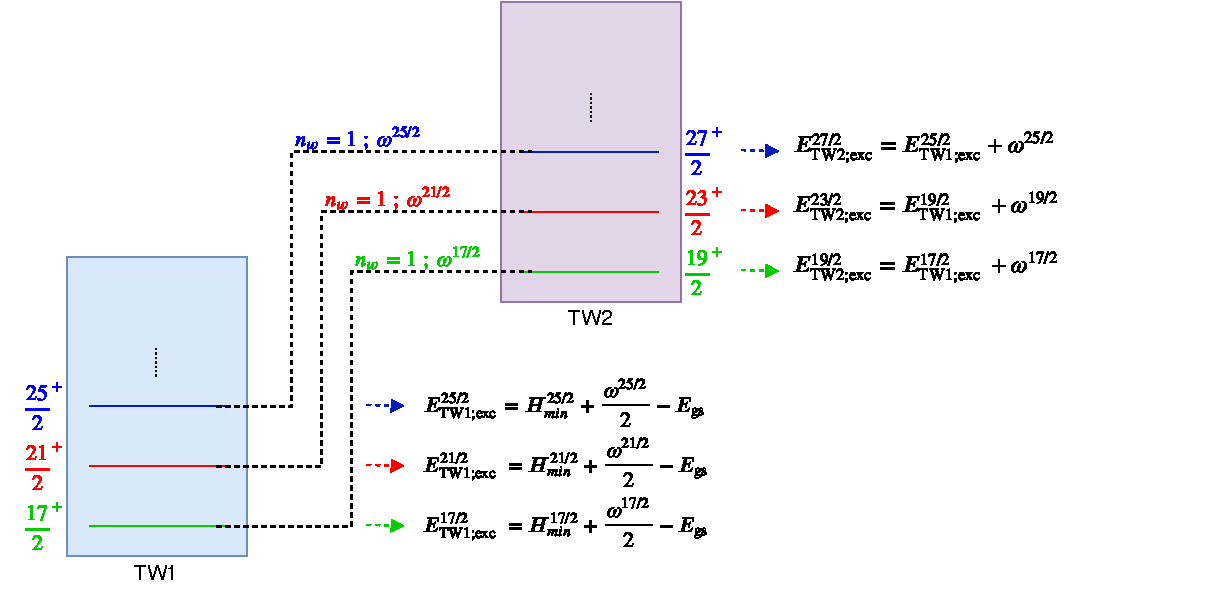
\includegraphics[scale=1]{images/pr135WobblingScheme1.pdf}
    \caption{TW1,TW2}
\end{figure}
\begin{figure}[h]
    \centering
    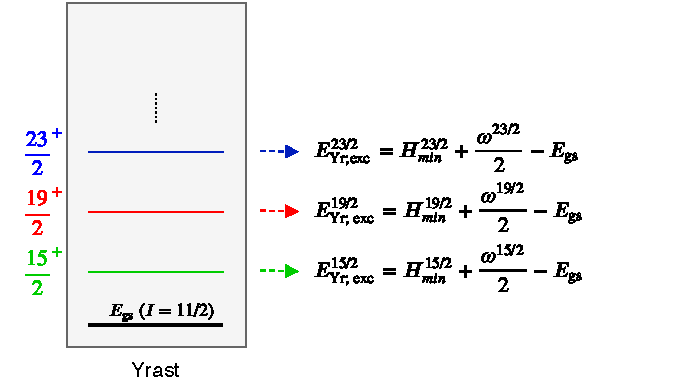
\includegraphics[scale=1]{images/pr135WobblingScheme2.pdf}
    \caption{YRAST}
\end{figure}
\section{Rezultate numerice}
Cu acest program am obtinut:
\begin{itemize}
    \item $\theta=-71^o$
    \item MOIs: $\mathcal{I}_1=89$, $\mathcal{I}_2=12$, $\mathcal{I}_3=48$
    \item $E_\text{RMS}=0.174452$
\end{itemize}
\begin{table}[h]
    \centering
    \begin{tabular}{ll}
    \hline
    \multicolumn{1}{|l|}{$I$} & \multicolumn{1}{l|}{$\omega^I$} \\ \hline
    \multicolumn{1}{|l}{7.5}  & \multicolumn{1}{l|}{0.239624} \\
    9.5                       & 0.295775                      \\
    11.5                      & 0.35077                       \\
    13.5                      & 0.405102                      \\
    15.5                      & 0.459018                      \\
    17.5                      & 0.512653                      \\
    19.5                      & 0.566089                      \\
    21.5                      & 0.619381                      \\
    23.5                      & 0.672562                      \\
    25.5                      & 0.725658                      \\
    27.5                      & 0.778687                      \\
    8.5                       & 0.267893                      \\
    10.5                      & 0.323378                      \\
    12.5                      & 0.378                         \\
    14.5                      & 0.432102                      \\
    16.5                      & 0.485864                      \\
    9.5                       & 0.295775                      \\
    11.5                      & 0.35077                       \\
    13.5                      & 0.405102                      \\
    15.5                      & 0.459018                      \\ \hline
    \end{tabular}
    \caption{Frecventele de wobbling pentru parametrii obtinuti, pentru toti spinii.}
    \end{table}
    \section{Reprezentari grafice}
    \subsection{Energii}
    Energiile de excitatie in functie de parametrii de fit.
    \begin{figure}[h]
        \centering
        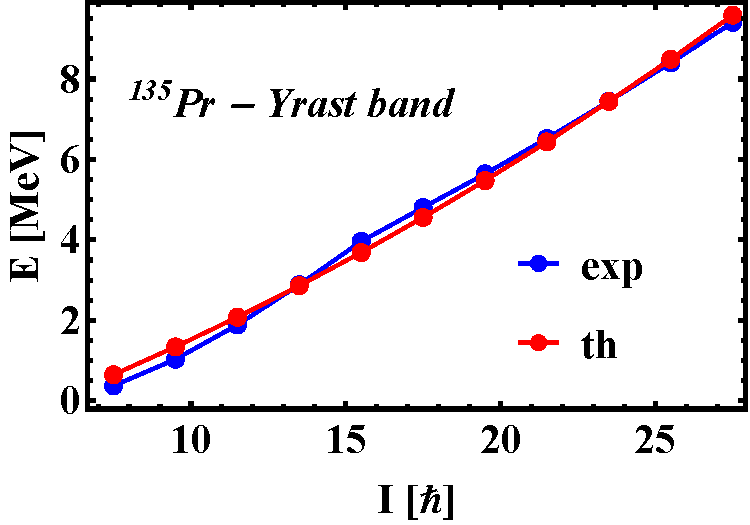
\includegraphics[scale=0.8]{images/tsd1.pdf}
        \caption{Banda yrast}
    \end{figure}
    \begin{figure}[h]
        \centering
        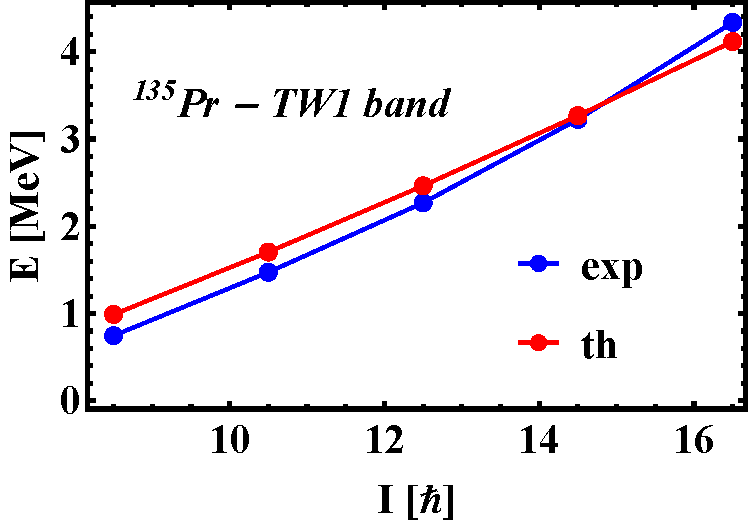
\includegraphics[scale=0.8]{images/tsd2.pdf}
        \caption{Banda TW1}
    \end{figure}
    \begin{figure}[h]
        \centering
        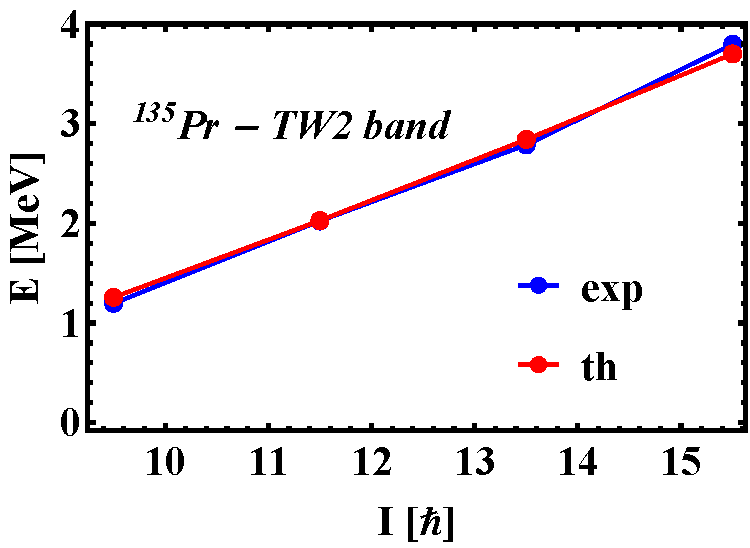
\includegraphics[scale=0.8]{images/tsd3.pdf}
        \caption{Banda TW2}
    \end{figure}
    \begin{figure}[h]
        \centering
        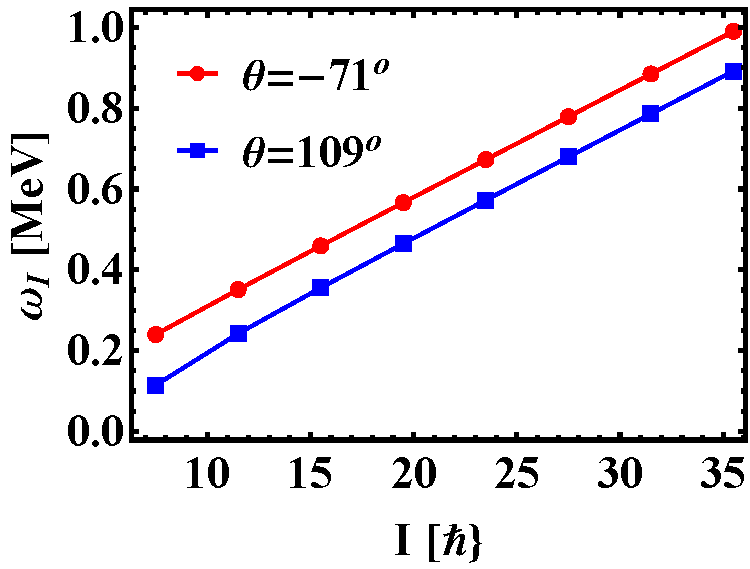
\includegraphics[scale=0.8]{images/omegas.pdf}
        \caption{Frecventele de wobbling pentru $\theta$ si $\theta+\pi$.}
    \end{figure}
\end{document}